%!TEX root=../main.tex


\section {A Proposed Architecture}
In this section we propose a high-level architecture of a ubiquitous monitoring ecosystem dedicated to accelerating vocabulary acquisition. 
% It is built around a platform dubbed Zeeguu. 
Figure \ref{fig:architecture} shows some of the main actors and components in our ecosystem.
 % detailing the {\em learning accelerator platform}.

\begin{figure}[h!]
	% \centering
	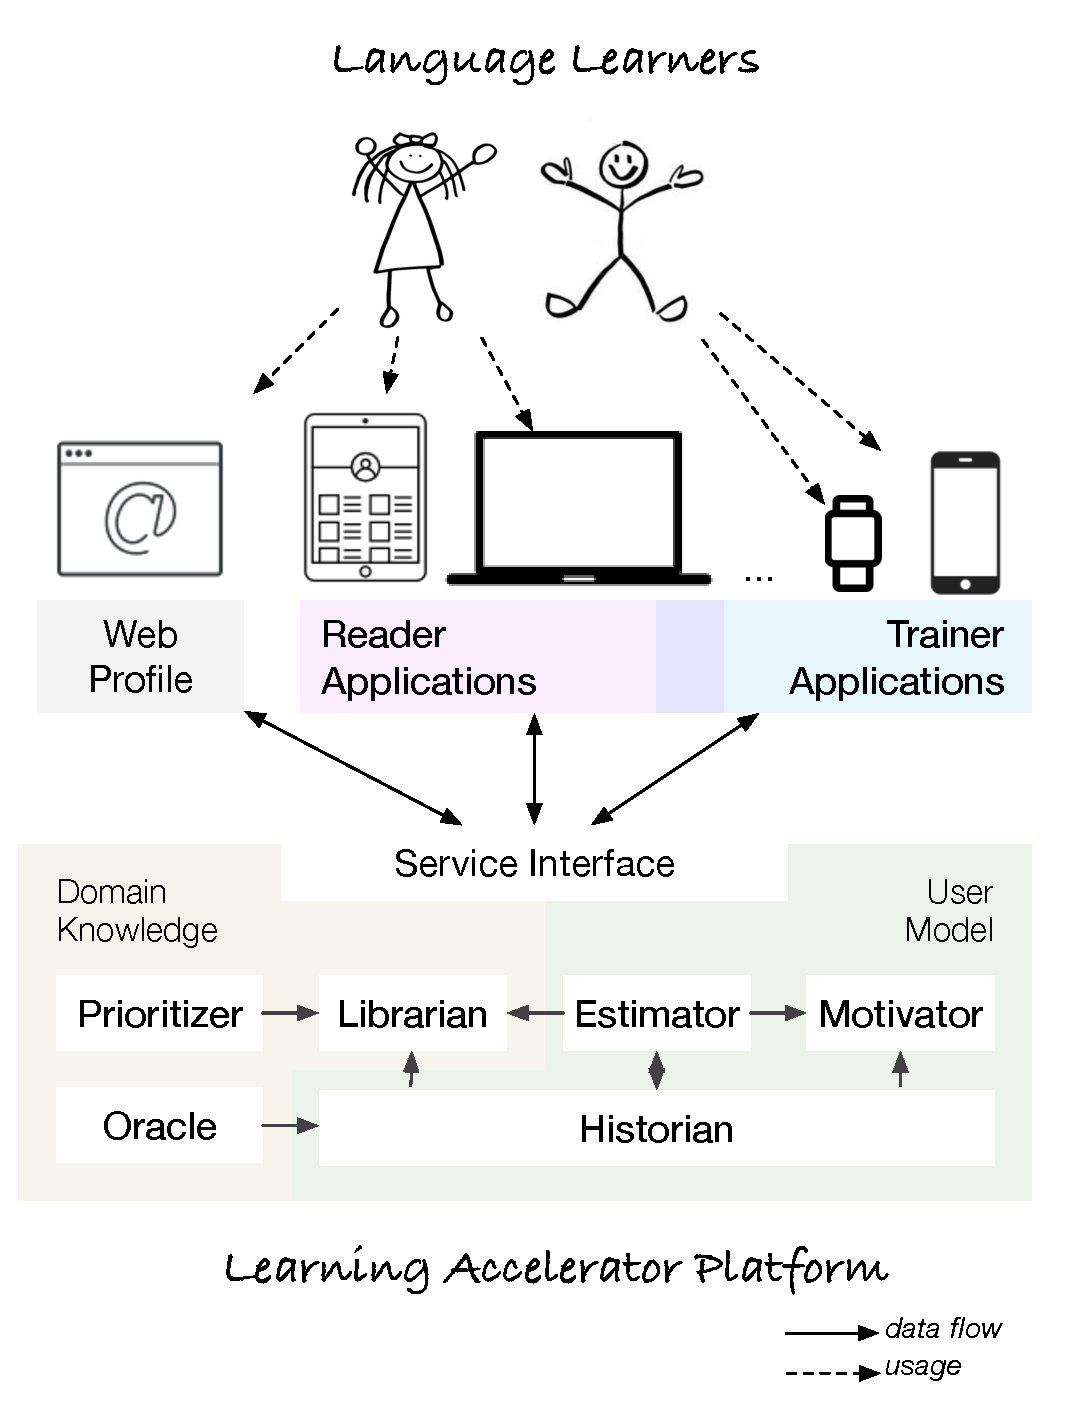
\includegraphics[width=0.99\linewidth]{images/zeeguu-architecture.pdf}
	\caption{A very high-level view of the architecture of an exemplar ubiquitous monitoring ecosystem}
	\label{fig:architecture}
\end{figure}

Only one category of actors is explicitly depicted -- the {\em language learners}. The {\em platform developers} and the {\em applicatoin developers} are missing from the picture. The latter are the makers of two types of applications: 

\begin{description}
	
	\item {\bf Reader Applications} facilitate the lecturing of materials in foreign languages. These applications have ideally two properties in common: 
		1) the usability of obtaining translations for unknown words 
		% in foreign language texts 
		is high (this is a quality attribute); 
		2) they report back to the platform information relevant for infering the current user knowledge\footnote{e.g., the looked-up words, their context, reading speed, etc.} (this is a functional requirement).

	\item {\bf Trainer Applications} provide exercises to accelerate the retention of individual words. Trainer applications have in common two functional properties: 
		1) they should request from the platform a list of words to be studied and 
		2) they must provide back to the platform information about how well the learner behaved with respect to a given word\footnote{e.g., the correctness of an answer, the time to answer, etc.}.

\end{description}

Note that the Reader and the Trainer applications need not necessarily be disjoint applications; instead one application could provide both functionalities.
% as the Figure \ref{fig:architecture} subtly suggests by overlapping the two corresponding blocks,


The {\em learning accelerator platform} sits at the core of the ecosystem since it stores and orchestrates the exchange of information between the various actors. It consists of six main components roughly divided into two categories: those related to domain knowledge and those related to user modeling.
% \footnote{The current implementation is not so crisply separated in components the figure suggests. This remains as future work}
The components are:


\newcommand {\archiblock}[1]{\item {\bf #1}}
\begin{enumerate}
	
		\archiblock{The Historian} is a data warehouse that sits at the core of a monitoring ecosystem. It records all the interactions of a user with knowledge based on the reports of Reader and Trainer applications.
		It stores the data in either a relational or a noSql database, depending on the type of data.

		\archiblock{The Oracle} is a service that {\em has all knowledge about the units of knowledge in the domain}. In our case it has knowledge of translations between many pairs of languages. It notifies the historian of every request it receives. 
		It uses adaptive strategies to choose between different backends that have different properties in terms of cost and quality.

		\archiblock{The Prioritizer} is a data mining focused component which aims at {\em ranking the information in the domain} based on a global view of its relative importance. It can be built based on statistical analysis of the learning patterns of the various leaners or based on a generic study of corpora in the target language.

		\archiblock{The Estimator} is a machine learning agent that {\em estimates the current knowledge of the learner} based on user-specific information received from the Historian and language-specific information received from the Prioritizer. It decides what are the most likely items that must be studied by the learner. 

% TODO: Re-read since this is completely refactored
		\archiblock {The Librarian} {\em provides reading recommendations wich are interesting to the learners while at the same being at the appropriate difficulty level}. It is a web crawler that uses natural language processing techniques but personalizes its results based on  information from the Estimator.

		% TODO: reference on gamificatoin? 
		\archiblock {The Motivator} is an agent that {\em uses gamification techniques to provide feedback that would keep the learner motivated}. It uses information 1) from the Historian to report on a learners {\em engagement} and 2) from the Estimator to provide feedback on the actual vocabulary acquisition {\em progress}. 

\end{enumerate}



% Somewhere, we still have to discuss the question of: 
% - How are we going to maintain this ecosystem? who will provide the data storage and translation facilities for the long run? 
% - What are the incentives for new players to join the ecosystem?
% - ... 


